\documentclass[a4paper, 11pt, russian]{article}

\usepackage[utf8]{inputenc}
\usepackage[T1, T2A]{fontenc}
\usepackage[english, russian]{babel}
\usepackage{indentfirst}
\usepackage{graphicx}
\usepackage{natbib}
\usepackage{caption, subcaption}
\usepackage[top=2cm, left=2cm, right=2cm, left=2cm]{geometry}
\usepackage{amsmath}
\usepackage{ragged2e}

\graphicspath{{Images/}}

\captionsetup[figure]{name = Рисунок, labelsep = endash}
\captionsetup[table]{name = Таблица, labelsep = endash, justification=raggedright, singlelinecheck=false}

\begin{document}
%Титульный лист
    \newcommand\tline[2]{$\underset{\text{#1}}{\text{\underline{\hspace{#2}}}}$}

\begin{titlepage}
	\centering
	{\fontsize{12pt}{5cm}\selectfont \bfseries Министерство образования и науки Российской Федерации} \\ \vspace{0.5cm}
	{\fontsize{7pt}{5cm}\selectfont ФЕДЕРАЛЬНОЕ ГОСУДАРСТВЕННОЕ АВТОНОМНОЕ ОБРАЗОВАТЕЛЬНОЕ УЧРЕЖДЕНИЕ ВЫСШЕГО ПРОФЕССИОНАЛЬНОГО ОБРАЗОВАНИЯ} \\ 
	\vspace{1cm}
	{\fontsize{12pt}{5cm}\selectfont \bfseries САНКТ-ПЕТЕРБУРГСКИЙ УНИВЕРСИТЕТ ИНФОРМАЦИОННЫХ ТЕХНОЛОГИЙ, МЕХАНИКИ И ОПТИКИ} \\ \vspace{1.5cm}

	{\fontsize{14pt}{5cm}\selectfont Кафедра \hspace{1cm} \underline{Систем Управления и Информатики}  \hspace{1cm} Группа \underline{Р3340}} \\ 
	\vspace{2cm}

	{\fontsize{20pt}{5cm}\selectfont \bfseries Лабораторная работа №7} \\
	{\fontsize{20pt}{5cm}\selectfont \bfseries “Анализ точности систем управления”} \\
	{\fontsize{14pt}{5cm}\selectfont Вариант - 2} \\
	\vspace{1.5cm}

	\flushleft

	{Выполнил \hspace{2cm} \underline{Алякин С.П.}\tline{(фамилия, и.о.)}{6.5cm} (подпись)} \\
	\vspace{2cm}

	{Проверил \hspace{2cm} \tline{(фамилия, и.о.)}{9cm} (подпись)} \\
	\vspace{5cm}

	"\underline{\hspace{0.7cm}}"\hspace{0.2cm}\underline{\hspace{2cm}}\hspace{0.2cm}20\underline{ 17 }г. \hspace{2cm} Санкт-Петербург, \hspace{2cm} 20\underline{ 17 }г. \\ \vspace{1cm}

	Работа выполнена с оценкой \hspace{1cm} \underline{\hspace{8cm}} \\ 
	\vspace{1cm}
	Дата защиты "\underline{\hspace{0.7cm}}"\hspace{0.2cm}\underline{\hspace{2cm}}\hspace{0.2cm}20\underline{ 17 }г.
		
\end{titlepage}

    \section{Введение}
    \subsection{Цель работы}
    Исследование точностных свойств систем управления.
    \subsection{Исходные данные}
    \begin{table}[ht!]
        \flushleft
        \caption{Исходные данные}
        \begin{tabular}{c|c|c|c}
            $W(s)$ & \multicolumn{3}{c}{Параметры сигнала задания} \\
            \hline
            $\displaystyle{\frac{3}{2,5s + 1}}$ & 2 & $2t$ & $0,5t^2$
        \end{tabular}
    \end{table}
    \clearpage
    \section{Исследование системы с астатизмом нулевого порядка}
    \begin{figure}[h!]
        \centering
        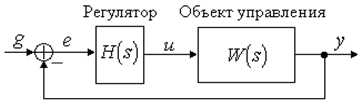
\includegraphics{0ast}
        \caption{Структурная схема моделируемой системы}
    \end{figure}
    Задана замкнутая система, представленная на рисунке 1, с регулятором $H(s) = k$ и передаточной функцией разомкнутого контура $W(s)=\displaystyle{\frac{3}{2,5s + 1}}$,схема моделирования которой представлена на рисунке 2.
    
    \begin{figure}[h!]
        \centering
        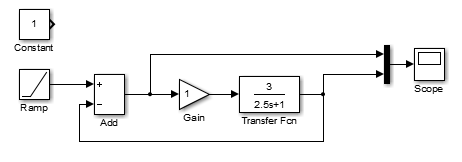
\includegraphics{0astScheme.PNG}
        \caption{Схема моделирования системы с астатизмом нулевого порядка}
    \end{figure}
    \subsection{Исследование стационарного режима работы: $g(t) = 2$.}
    Рассчисаем предельное значение установившейся ошибки: $$\varepsilon = \lim_{s\to0} s\frac{1}{1 + H(s)W(s)}G(s) = \lim_{s\to0} s\frac{1}{1 + \frac{3k}{2,5s + 1}}\cdot\frac{2}{s} = \lim_{s\to0} \frac{5s + 2}{2,5s + 3k + 1} = \frac{2}{1 + 3k}$$\\
    При $k = 1: \varepsilon = 0,5$\\
    При $k = 5: \varepsilon = 0,125$\\
    При $k = 10: \varepsilon = \displaystyle{\frac{2}{31}} \approx 0,065$\\
    
    По полученным графикам, представленным на рисунке 3, видно, что полученные при моделировании значения ошибки равны рассчитанным аналитически.\\
    \begin{figure}[h!]
        \centering
        \begin{subfigure}[h]{0.7\textwidth}
            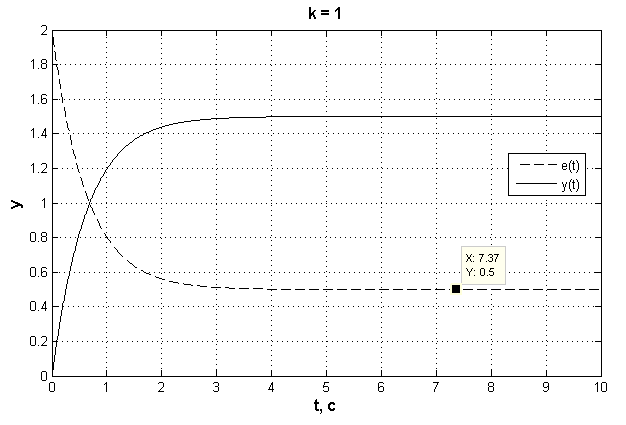
\includegraphics[width = \textwidth]{constInput0ast1k.png}
            \\
            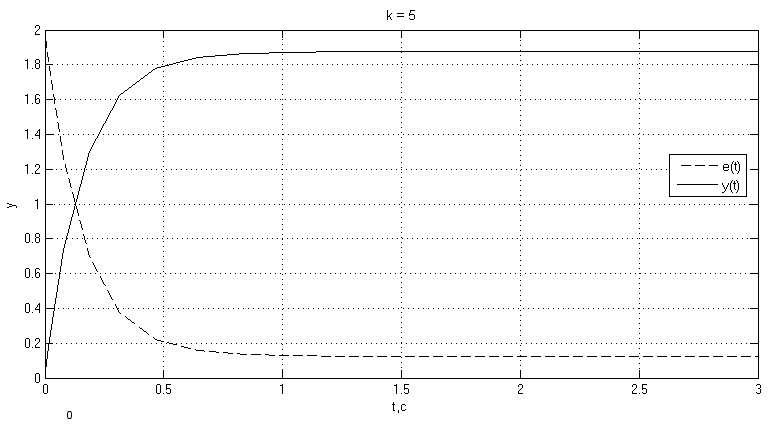
\includegraphics[width = \textwidth]{constInput0ast5k.png}
            \\
            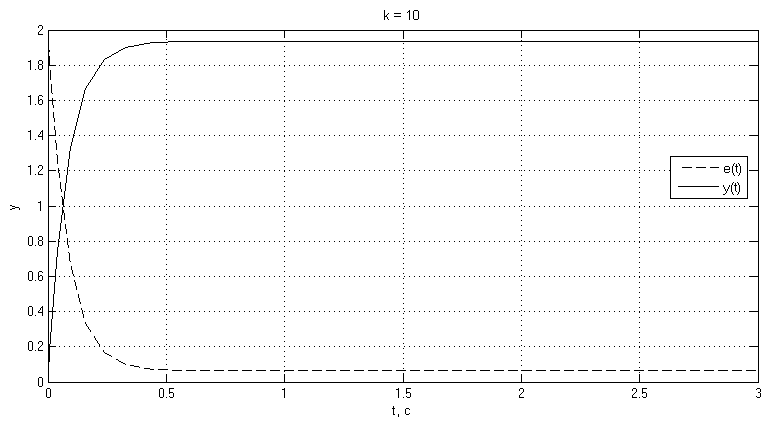
\includegraphics[width = \textwidth]{constInput0ast10k.png}
        \end{subfigure}
        \caption{Переходные процессы при $g(t) = 2$}
    \end{figure}
    \vspace{1.5cm} %Иначе подраздел начинается до графиков
    \subsection{Исследование режима движения с постоянной скоростью: $g(t) = 2t$}
    Так как система статична, то ошибка при линейном входном воздействии должна стремиться к $\infty$, что и показанно эксперементально на рисунке 4.
    
    %Делаю как отдельные фигуры, чтобы графики могли переноситься на другую страницу по одному
    \begin{figure}[h!]
        \centering
        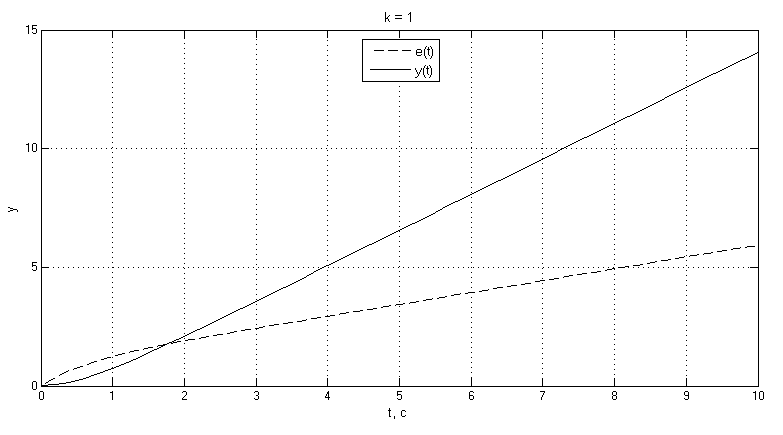
\includegraphics[scale = 0.75]{vInput0ast1k.png}
    \end{figure}
    \begin{figure}[h!]
        \centering
        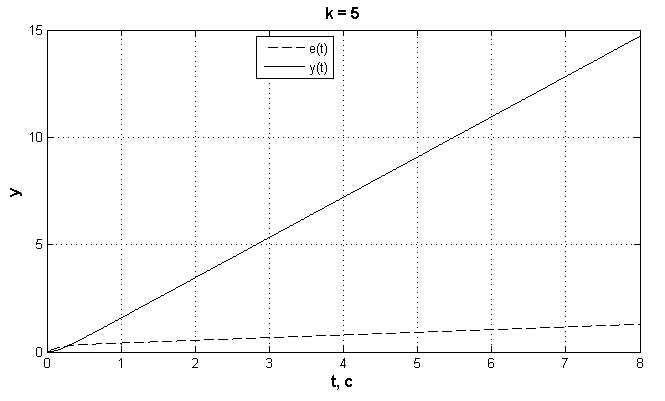
\includegraphics[scale = 0.75]{vInput0ast5k.png}
    \end{figure}
    \begin{figure}[ht!]
        \centering
        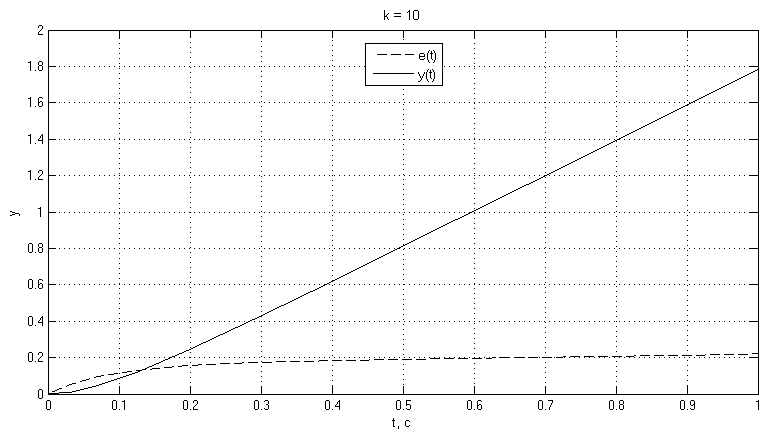
\includegraphics[scale = 0.75]{vInput0ast10k.png}
        \caption{Переходные процессы при $g(t) = 2t$}
    \end{figure}
    \clearpage
    \section{Исследование системы с астатизмом первого порядка}
    Структурная схема моделируемой системы представлена на рисунке 1, где $H(s) = \displaystyle{\frac{k}{s}}, W(s) = \displaystyle{\frac{3}{2,5s + 1}}$.
    
    \begin{figure}[h!]
        \centering
        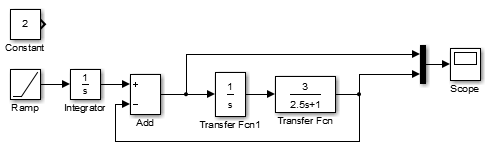
\includegraphics{1astScheme.PNG}
        \caption{Схема моделирования системы с астатизмом первого порядка}
    \end{figure}
    \subsection{Исследование стационарного режима работы: $g(t) = 2$}
    Аналитически рассчитанное значение установившейся ошибки равно $$\varepsilon = \lim_{s\to0} s\frac{1}{1 + H(s)W(s)}G(s) = \lim_{s\to0} \frac{2}{1 + \frac{W(s)}{s}} = \lim_{s\to0} \frac{2s(2,5s + 1)}{s(2,5s + 1) + 3} = \frac{0}{3} = 0,$$ что и показанно эксперементально на рисунке 6.
    
    \begin{figure}[hp!]
        \centering
        \begin{subfigure}[h]{0.9\textwidth}
            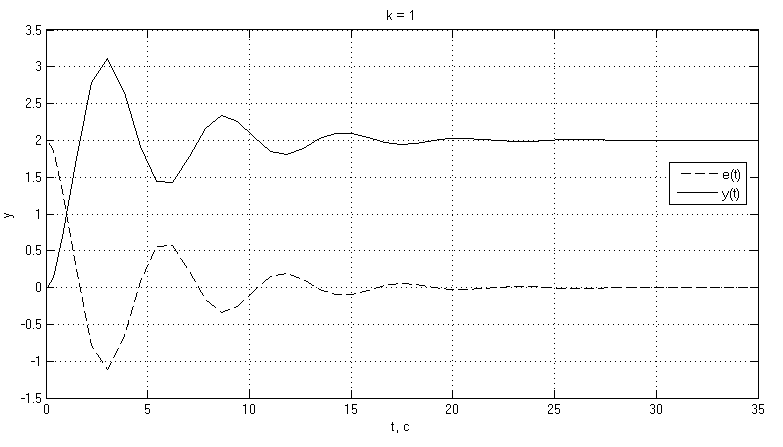
\includegraphics[width = \textwidth]{constInput1ast1k.png}\\
            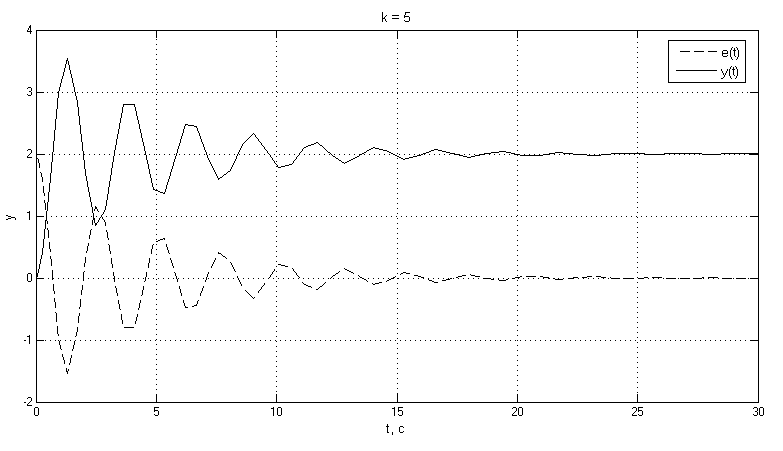
\includegraphics[width = \textwidth]{constInput1ast5k.png}\\
            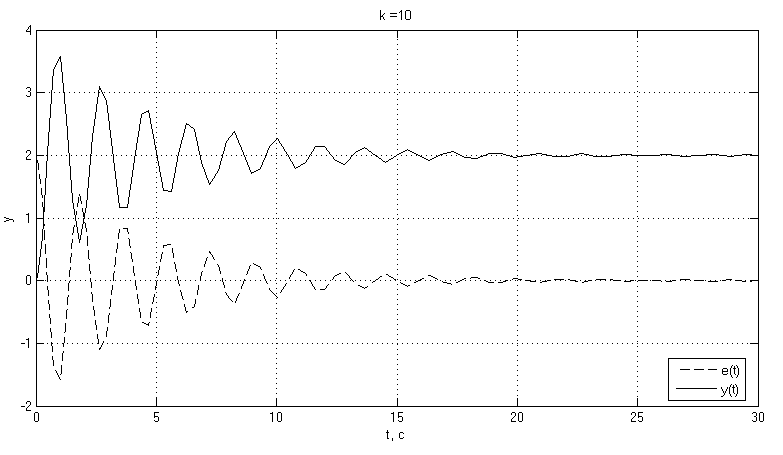
\includegraphics[width = \textwidth]{constInput1ast10k.png}
        \end{subfigure}
        \caption{Переходные процессы при $g(t) = 2$}
    \end{figure}
    \clearpage
    \subsection{Исследование режима движения с постоянной скоростью: $g(t) = 2t$}
    Рассчитаем предельное значение ошибки для системы при $g(t) = 2t$: $$\varepsilon = \lim_{s\to0} s\frac{1}{1 + H(s)W(s)}G(s) = \lim_{s\to0} \frac{s}{1 + \frac{3k}{s(2,5s + 1)}}\cdot\frac{2}{s^2} = \lim_{s\to0} \frac{2(2,5s + 1)}{2,5s^2 + s + 3k} = \frac{2}{3k}$$\\
    При $k = 1: \varepsilon = \displaystyle{\frac{2}{3}} \approx 0,67$\\
    При $k = 5: \varepsilon = \displaystyle{\frac{2}{15}} \approx 0,13$\\
    При $k = 10: \varepsilon = \displaystyle{\frac{1}{15}} \approx 0,067$\\
    
    По полученным графикам, представленным на рисунке 7, видно, что полученное при симуляции значения ошибки равны рассчитанным аналитически.
    \begin{figure}[h!]
        \centering
        \begin{subfigure}{0.65\textwidth}
            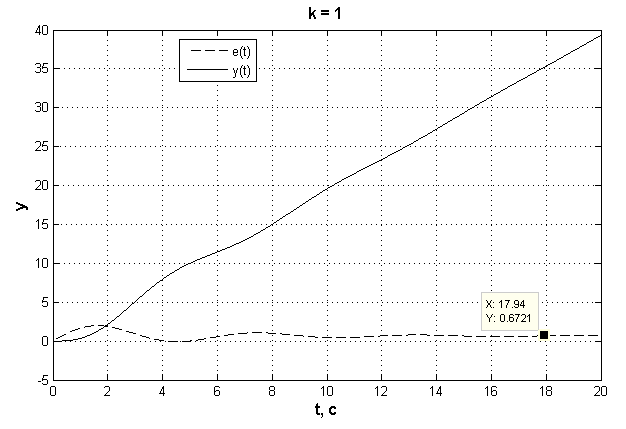
\includegraphics[width = \textwidth]{vInput1ast1k.png}
            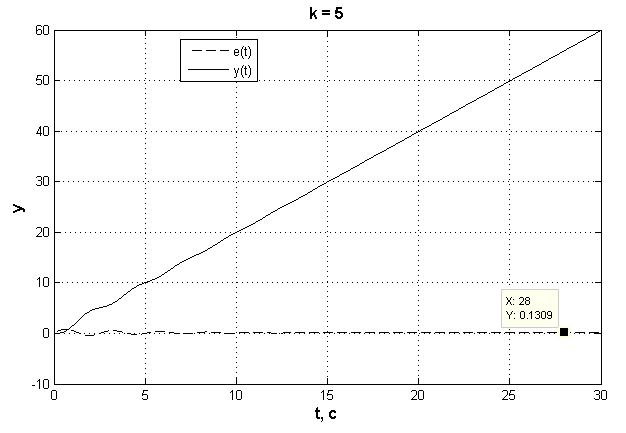
\includegraphics[width = \textwidth]{vInput1ast5k.png}
            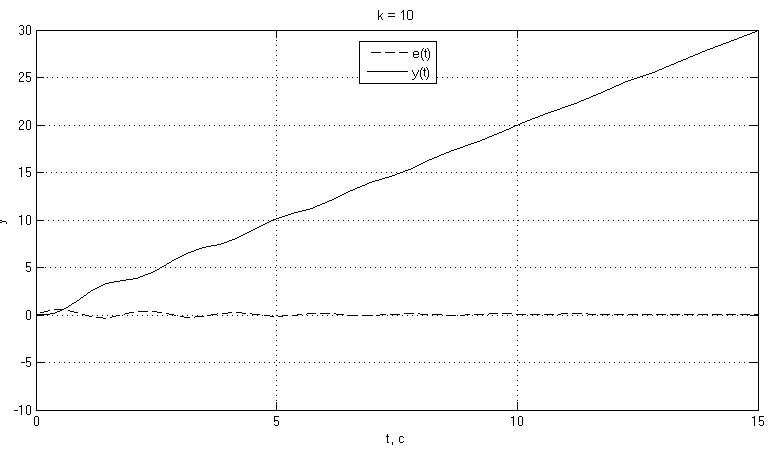
\includegraphics[width = \textwidth]{vInput1ast10k.png}
        \end{subfigure}
        \caption{Переходные процессы при $g(t) = 2t$}
    \end{figure}
    
    \subsection{Исследование режима движения с постоянным ускорением: $g(t) = 0,5t^2$}
    При движении с постоянным ускорением ошибка для системы с астатизмом первого порядки должна стремиться к $\infty$, что и показанно на рисунке 8, на котором представленны результаты работы математической модели соответствующей системы.
    \begin{figure}[ht!]
        \centering
        \begin{subfigure}{0.75\textwidth}
            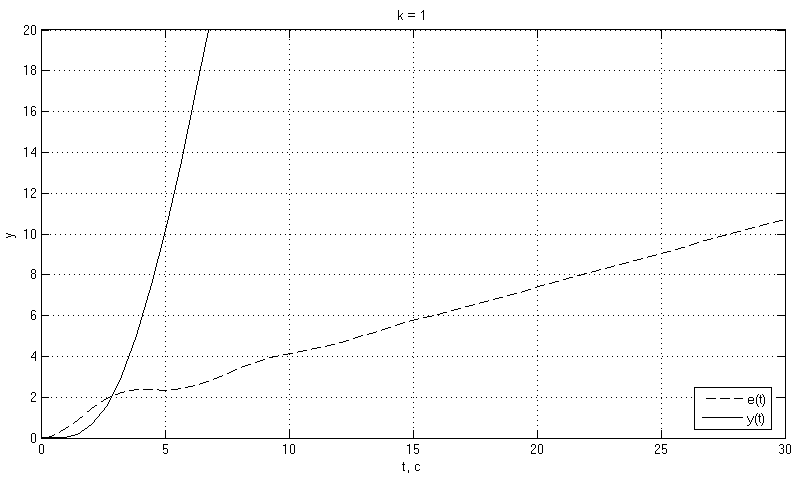
\includegraphics[width = \textwidth]{aInput1ast1k.png}
            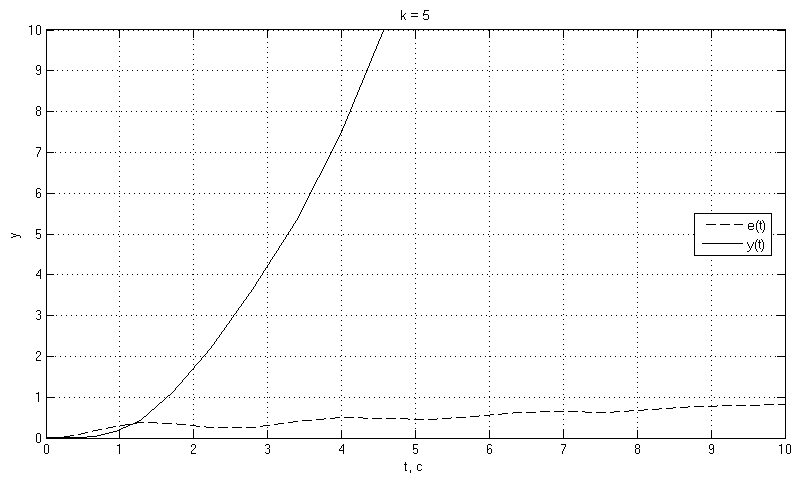
\includegraphics[width = \textwidth]{aInput1ast5k.png}
            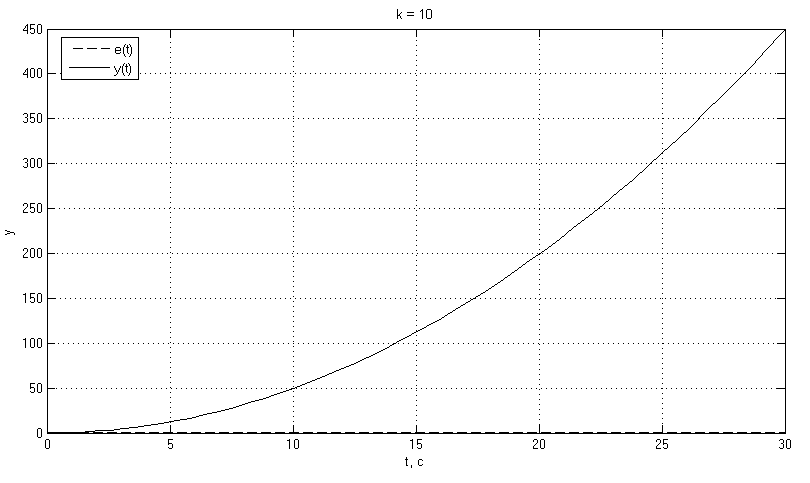
\includegraphics[width = \textwidth]{aInput1ast10k.png}
        \end{subfigure}
        \caption{Переходные процессы при $g(t) = 0,5t^2$}
    \end{figure}
    \clearpage
    \section{Исследование влияний внешних возмущений}
    Схема моделирования возмущённой системы представлена на рисунке 9, где $W(s) = \displaystyle{\frac{3}{2,5s + 1}}, f_1 = 0,5, f_2 = 0,5.$\\
    \begin{figure}[ht!]
        \centering
        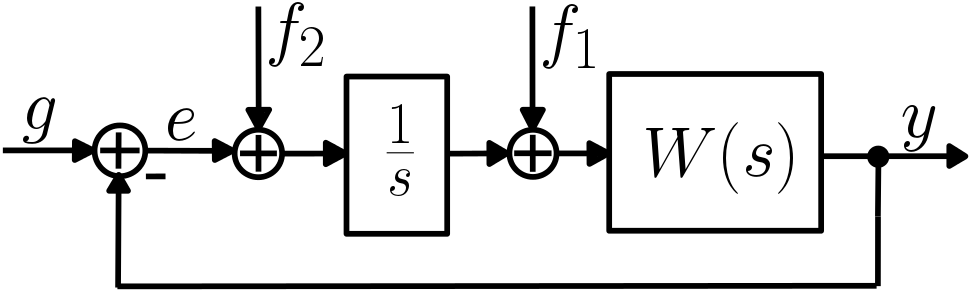
\includegraphics{disturbScheme}
        \caption{Структурная схема возмущённой системы}
    \end{figure}
    
    Схема моделированя соответствующей возмущённой системы представленна на рисунке 10.
    
    \begin{figure}[h!]
        \centering
        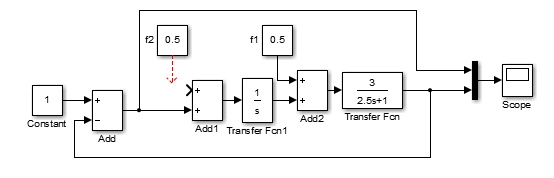
\includegraphics{dstScheme.PNG}
        \caption{Схема моделирования возмущённой системы}
    \end{figure}
    
    Функция ошибки равна $$e = \frac{g - f_1W(s) - f_2W(s)\displaystyle{\frac{1}{s}}}{1 + W(s)\displaystyle{\frac{1}{s}}} = \frac{g - f_1\displaystyle{\frac{3}{2,5s + 1}} - f_2\displaystyle{\frac{3}{(2,5s + 1)s}}}{1 + \displaystyle{\frac{3}{(2,5s + 1)s}}} = \frac{g(2,5s^2 + s) - 3sf_1 - 3f_2}{2,5s^2 + s + 3},$$\\
    тогда предельное значение ошибки при $g(t) = 1$ $$\varepsilon = \lim_{s\to0} \frac{2,5s^2 + s - 3sf_1 - 3f_2}{2,5s^2 + s + 3} = \frac{-3f_2}{3} = -f_2.$$
    Получается, что при постоянных возмущениях $f_1(t)$ и $f_2(t)$ ошибка будет равняться $-f_2$.
    \subsection{Полагаем $f_2(t) = 0$ и $g(t) = 1(t)$}
    Исходя из аналитически рассчитанного выражения для ошибки, предельное значение ошибки при заданных параметрах должно равнятся 0. Что и продемонстрированно на графике, представленном на рисунке 11.
    
    \begin{figure}[ht!]
        \centering
        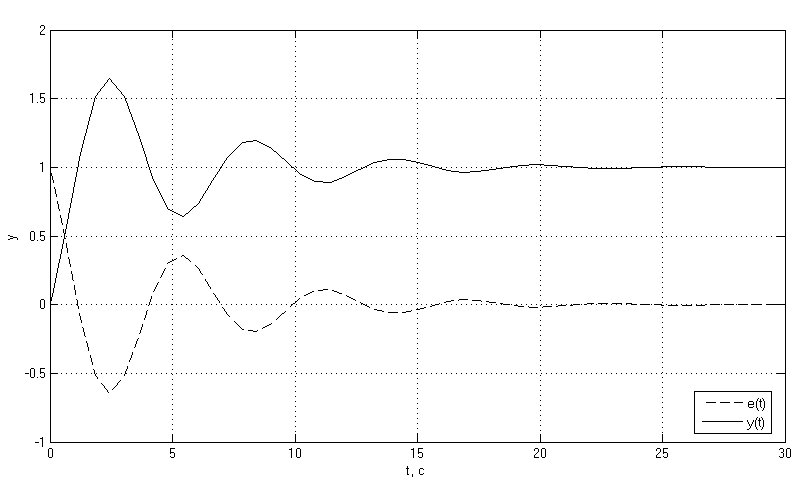
\includegraphics[scale = 0.75]{disturbance1.png}
        \caption{График переходного процесса с возмущением $f_1$}
    \end{figure}
    \vspace{4.5cm}
    \subsection{Полагаем $f_1 = 0$ и $g(t) = 1(t)$}
    По рассчитанному ранее значению выражению для ошибки, установившееся значение ошибки должно быть равно $-f_2$, что и показывают результаты математического моделирования, представленные на рисунке 12.
    
    \begin{figure}[ht!]
        \centering
        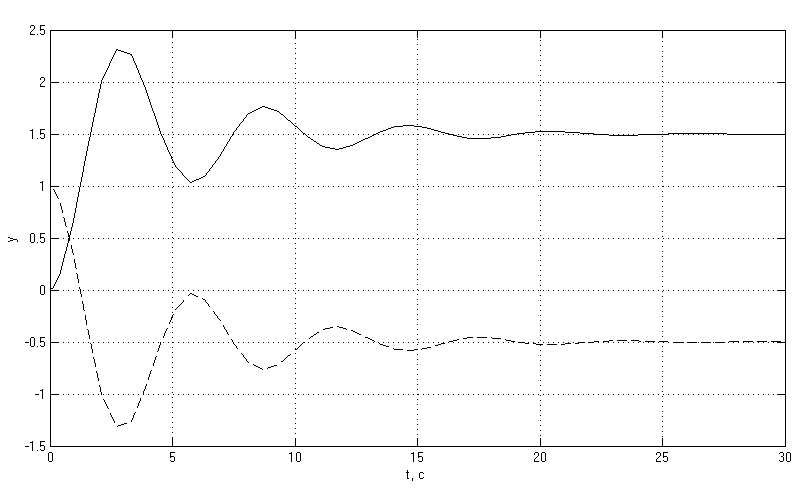
\includegraphics[scale = 0.7]{disturbance2.png}
        \caption{График переходного процесса с возмущением $f_2$}
    \end{figure}
    
    \section{Исследование установившейся ошибки при произвольном входном воздействии}
    Структурная схема представлена на рисунке 1, где $H(s) = 1, W(s) = \displaystyle{\frac{3}{2,5s + 1}}$, а задающее воздействие $g(t) = 0,2t^2 + \sin{0,5t}$.
    \subsection{Результаты моделирования}
    В результате моделирования заданной системы был получен график, представленный на рисунке 14. Из него видно, что предельное значение ошибки стремится к $\infty$. Схема моделирования системы представленна на рисунке 13.
    \begin{figure}[h!]
        \centering
        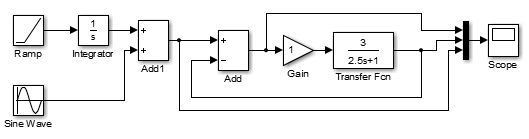
\includegraphics[scale = 1]{customSourceScheme.PNG}
        \caption{Схема моделирования системы с производным входным воздействием}
    \end{figure}
    
    \begin{figure}[h!]
        \centering
        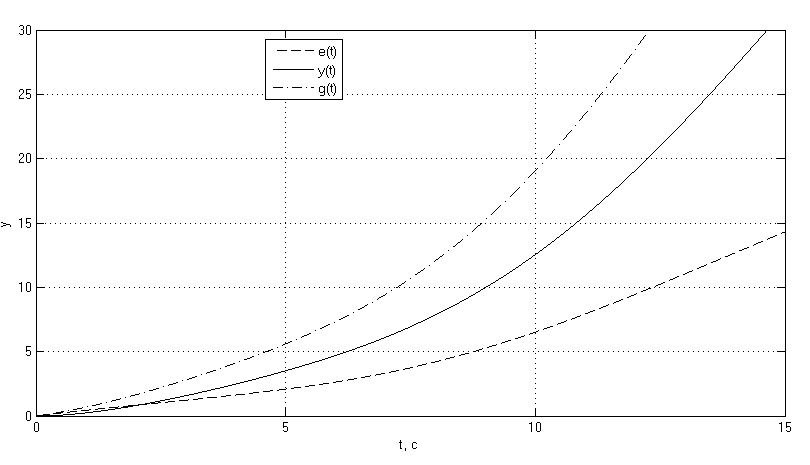
\includegraphics[scale = 0.75]{customInput.png}
        \caption{Результат работы системы при входном воздействии $g(t) = 0,2t^2 + \sin{0,5t}$}
    \end{figure}
    \vspace{2cm}
    \subsection{Получение приближенного выражения для ошибки}
    Разложим передаточную функцию замкнутой системы $\Phi_e(s) = \displaystyle{\frac{1}{1 + W(s)}}$ в ряд Тейлора, сохранив только первые 3 члена. 
    $$\Phi_e(s) = \frac{2,5s + 1}{2,5s + 4} \approx \frac{1}{4} + 0,47s - 0,29s^2,$$
    тогда получаем выражение установившейся ошибки при произвольном входном воздействии
    $$e_y(t) = 0,25g(t) + 0,47\frac{d}{dt}g(t) - 0,29\frac{d^2}{dt^2}g(t).$$
    Найдём производные $g(t)$:
    $$g(t) = 0,2t^2 + \sin{0,5t};$$
    $$\frac{d}{dt}g(t) = 0,4t + 0,5\cos{0,5t};$$
    $$\frac{d^2}{dt^2}g(t) = 0,4 - 0,25\sin{0,5t},$$
    тогда выражение ошибки $e_y(t)$ принимает вид
    $$e_y(t) = 0,05t^2 + 0,25\sin{0,5t} + 0,188t + 0,235\cos{0,5t} - 0,116 + 0,0725\sin{0,5t} =$$
    $$= 0,05t^2 + 0,188t - 0,116 + 0,3225\sin{0,5t} + 0,235\cos{0,5t}$$
    Из полученного выражения видно, что, с течением времени, ошибка стремится к $\infty$. Чтобы определить, совпадает ли расчитанная ошибка с моделированной, построим их на одном графике,еоторый представлен на рисунке 15.
    \begin{figure}[ht!]
        \centering
        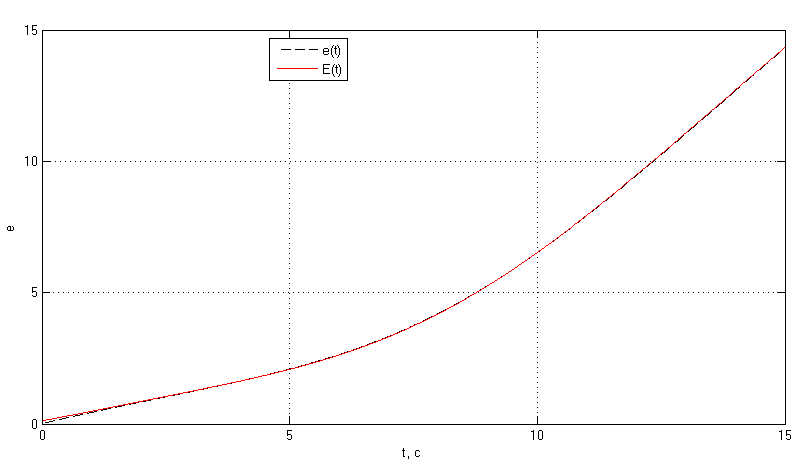
\includegraphics[scale = 0.75]{customInputTaylor.png}
        \caption{Значения ошибок при произвольном входящем воздействии, где $e(t)$ -- получена при моделировании, $E(t)$  -- рассчитана аналитически}
    \end{figure}
    \vspace{1.5cm}
    \section{Вывод}
    В данной работе были исследованны способы повышения точности исследуемой системы. Было показанно, что на значение установившейся ошибки можно повлиять, изменяя степень астатизма системы и/или коэффициент усиления разомкнутой системы.
    
    Кроме того было показанно, что порядок астатизма системы по входящему воздействию может не соответсвовать порядку астатизма по возмущению.
    
    Так же было полученно и расчитанно аналитически значение ошибки системы при произвольном входном воздействии.
\end{document}